\documentclass{article}

\usepackage[T1]{fontenc}
\usepackage[utf8]{inputenc}
\usepackage{graphicx}
\usepackage{booktabs, siunitx}
\usepackage{tikz}
\usepackage{tikz-qtree}
\usepackage{pifont}
\usepackage[margin=0.90in]{geometry}
\usepackage{etoolbox,titling}
\usepackage{enumitem}
\usepackage{fancyhdr}
\usepackage{soulutf8}
\usepackage{tcolorbox}
\tcbuselibrary{skins}

\definecolor{boxTitle}{HTML}{fff79a}
\definecolor{boxBackground}{HTML}{fffce0}
\definecolor{boxFrame}{HTML}{f1e2b8}


\definecolor{boxTitle2}{HTML}{b3ffda}
\definecolor{boxBackground2}{HTML}{e6f2ff}
\definecolor{boxFrame2}{HTML}{b3d7ff}

\definecolor{boxTitle3}{HTML}{ff794d}
\definecolor{boxBackground3}{HTML}{ffe6e6}
\definecolor{boxFrame3}{HTML}{ffb399}

\definecolor{boxTitle4}{HTML}{d7d7c1}
\definecolor{boxBackground4}{HTML}{ebebe0}
\definecolor{boxFrame4}{HTML}{c3c3a2}


\tcbset{box1/.style={
    enhanced, fonttitle=\bfseries,
    colback=boxBackground, colframe=boxFrame,
    coltitle=black, colbacktitle=boxTitle,
    attach boxed title to top left={xshift=0.3cm,
                                    yshift*=-\tcboxedtitleheight/2}
  }
}
\newtcolorbox{box1}[1][]{box1, #1}

\tcbset{box2/.style={
    enhanced, fonttitle=\bfseries,
    colback=boxBackground2, colframe=boxFrame2,
    coltitle=black, colbacktitle=boxTitle2,
    attach boxed title to top left={xshift=0.3cm,
                                    yshift*=-\tcboxedtitleheight/2}
  }
}
\newtcolorbox{box2}[1][]{box2, #1}

\tcbset{box3/.style={
    enhanced, fonttitle=\bfseries,
    colback=boxBackground3, colframe=boxFrame3,
    coltitle=black, colbacktitle=boxTitle3,
    attach boxed title to top left={xshift=0.3cm,
                                    yshift*=-\tcboxedtitleheight/2}
  }
}
\newtcolorbox{box3}[1][]{box3, #1}

\tcbset{box4/.style={
    enhanced, fonttitle=\bfseries,
    colback=boxBackground4, colframe=boxFrame4,
    coltitle=black, colbacktitle=boxTitle4,
    attach boxed title to top left={xshift=0.3cm,
                                    yshift*=-\tcboxedtitleheight/2},
    boxed title style={
      before upper=\hspace*{0.5cm}, % reserve space for the image
      overlay={
       \node at ([xshift=0.1cm]frame.west)
         {\includegraphics[scale=0.65]{bc-loupe}};
      }
    }
  }
}

\newtcolorbox{box4}[1][]{box4, #1}

\pagestyle{fancy}
\fancyhf{}
\rhead{Open Targets Genetics}
\lhead{Relazione presentazione NAR}
\rfoot{Pagina \thepage}
\lfoot{Bioinformatica - A.A. 2021/22}
\usetikzlibrary{trees}
\tikzstyle{every node}=[draw=black,thick,anchor=west]


\begin{document}
\newcommand\tab[1][0.3cm]{\hspace*{#1}}


\begin{titlepage}
    \begin{center}
        \vspace*{1cm}
            
        \Huge
        \textbf{Laboratorio di Bioinformatica - Presentazione NAR}
            
        \vspace{0.5cm}
        \LARGE
        Relazione associata
            
        \vspace{1.5cm}
            
        \textbf{Chiara Solito e Aurelia Timis}

        \vspace{0.8cm}

            
        \Large
        Corso di Laurea in Bioinformatica\\
        Università degli studi di Verona\\
        A.A. 2021/22
            
    \end{center}
\end{titlepage}
La presente è una relazione riguardante la presentazione del database Open Targets Genetics. È stata scritta nell'ambito dei database trattati in \textit{Nucleic Acids Research, 2021, Vol. 49, Database issue D1-D9}, per il corso di \textbf{Laboratorio di Bioinformatica} del CdS in Bioinformatica (Università degli Studi di Verona), A.A. 2021/2022.\\
Insieme a questo documento in formato PDF viene fornito anche il codice \LaTeX  con cui è stato generato.
\tableofcontents
\thispagestyle{empty}
\newpage
\thispagestyle{empty}
\section{Introduzione}
\subsection{Lessico e nozioni di base}
\subsection*{Nozioni di Statistica}
\paragraph{Single Evidence Score}
Tra i livelli di Evidenza, anche definiti come gerarchia dell'evidenza, assegnati agli studi, basandosi sulla qualità metodologica della loro progettazione, validità e applicabilità alla cura del paziente: è il sesto livello di evidenza - Evidenza da un singolo studio descrittivo o qualitativo.
\paragraph{Proxy}Un proxy è una misura indiretta del risultato desiderato che è esso stesso fortemente correlato a quel risultato. È comunemente usato quando le misure dirette del risultato non sono osservabili e/o non disponibili.
\paragraph{Credible Sets}\textit{Set Credibili}\\sono l'insieme più piccolo di varianti, selezionate in modo tale che la loro stima di copertura rettificata soddisfi la copertura del target. Ad esempio: in letteratura, gli autori in genere riferiscono di aver trovato un insieme credibile al 90\% di cui sono fiduciosi almeno al 90\% contenga la vera variante causale.
\paragraph{PP - Posterior Probability}\textit{Probabilità a posteriori}\\In statistica bayesiana, la probabilità a posteriori di un evento aleatorio o di una proposizione incerta, è la probabilità condizionata che è assegnata dopo che si è tenuto conto dell'informazione rilevante o degli antefatti relativi a tale evento aleatorio o a tale proposizione incerta. Similmente, la distribuzione di probabilità a posteriori è la distribuzione di una quantità incognita, trattata come una variabile casuale, condizionata sull'informazione posta in evidenza da un esperimento o da un processo di raccolta di informazione rilevanti (es. un'ispezione, un'indagine conoscitiva, ecc.).
\paragraph{P-Value}La probabilità, per un'ipotesi supposta vera (ipotesi nulla), di ottenere risultati ugualmetnte o meno compatibili, di quelli osservati durante i test, con la suddetta ipotesi.
\par\noindent\rule{\textwidth}{0.4pt}
\subsection*{Nozioni sui GWAS}
\paragraph{GWAS}\textit{Genome Wide Association Study}\\Un approccio della ricerca genetica per associare, a specifiche variazioni genetiche, particolari malattie.
\paragraph{Varianti Causali}Nell'ambito degli studi di associazione, le varianti genetiche responsabili del segnale di associazione in un locus sono indicate nella letteratura come VARIANTI CAUSALI. Esse hanno un effetto biologico sul fenotipo.
\paragraph{Lead Variant}La variante col miglior p-value per combinazioni gene/fenotipo significative.
\paragraph{Tag Variants}Varianti rappresentative in una regione del genoma con un alto linkage disequilibrium.
\paragraph{Trait-Associated Loci}\textit{Loci tratto associati}\\Un locus a cui è associao un particolare tratto fenotipico.
\paragraph{QTL}\textit{Quantitative trait loci}\\
    Un locus dei caratteri quantitativi (ovvero tratti che possono essere studiati e indagati mediante parametri numerici) è un locus che si correla con la variazione di un tratto quantitativo nel fenotipo di una popolazione di organismi.
\paragraph{Linkage Disequilibrium} Linkage disequilibrium (LD) è l'associazione non casuale di alleli di diversi loci. Non esiste una singola statistica migliore che quantifica l'entità di LD. Sono state proposte diverse statistiche utili per scopi diversi.
\paragraph{Fine Mapping}Dal momento che i risultati dei GWAS non sempre ci danno una sintesi completa delle statistiche, e avendo a disposizione solo le Variant Lead, dobbiamo ampliare le informazioni con le Variants Tag, in modo da avere un insieme più completo.\\Il fine mapping è uno dei metodi con quei viene eseguita questa operazione: è una tecnica dei GWAS per identificare la varianti genetiche che possono influenzare causalmente il tratto esaminato, in particolare cerca di determinare la variante genetica responsabile della malattia o del fenotipo analizzato.
\paragraph{Linkage Disequilibrium Espansione}
Sappiamo che il genoma viene ereditato a blocchi e ogni blocco è definito da un aplotipo, che a sua volta è definito da un insieme di SNPs. OTG prende in considerazione l'LD perchè pazienti che hanno ereditato lo stesso segmento cromosomico, definito dal medesimo aplotipo, possono aver ereditato anche la stessa mutazione. L'LD ha persmesso nelle analisi di associazioni, di studiare soo gli SNPs necessari a identificare il blocco di DNS in disequilibrium. 

\section{Open Targets Genetics}

\subsection{Cos'è Open Targets Genetics?}
Open Target Genetics è l'ultima \textit{release} della piattaforma Open Targets: una \textit{partnership} tra pubblico e privato che utilizza i dati genetici e genomici umani per l'identificazione sistematica e la prioritizzazione dei bersagli farmacologici.\\
Il portale offre tre caratteristiche al fine di mettere in luce le associazioni tra \textbf{geni, varianti e tratti}:
\begin{itemize}
    \item Sfogliare e classificare le associazioni di geni e varianti identificate dalla pipeline di punteggio \textbf{Locus-to-Gene (L2G)}
    \item Scoprire set credibili per associazioni di varianti e tratti basati sulla pipeline di analisi di \textit{fine mapping}.
    \item Esplorare e confrontare gli studi della UK BioBank, di FinnGen e del catalogo GWAS utilizzando lo strumento di confronto multi-tratto
\end{itemize} 

\begin{box3}
    [title={\textbf{La novità di OTG}}]
    {La maggior parte delle varianti, individuate attraverso i GWAS, si trova nella parte non codificante del genoma: ciò suggerisce che tali varianti vadano ad intaccare tratti complessi, alterando l'espressione dei geni vicini, attraverso meccanismi di regolazione, e influenzando in maniera significativa le malattie studiate dai GWAS. 
    Identificare un gene causale è difficile poiché bisogna integrare dati dai GWAS con dati di trascrittomica, proteomica ed epigenomica prendendo in considerazione un'ampia tipologia cellulare o tissutale.In assenza di un portale già esistente che consenta di rispondere sistematicamente a un'ampia gamma di domande biologiche, è stato costruito OTG sulla base della tecnologia più recente per consentire di aggiungere e sfogliare facilmente i dati.}
\end{box3}

\subsection{L'Obiettivo}
Identificare bersagli farmacologici per lo sviluppo di medicinali sicuri ed efficaci è una priorità per l'industria farmaceutica; lo sviluppo di farmaci porta spesso a perdite di tempo e risultati fallimentari.
I \textbf{farmaci con targets} che hanno evidenziato prove genetiche per associazioni a malattie, hanno dimostrato di essere vincenti nello sviluppo clinico. Ecco che, una sistematica valutazione di associazioni genetiche a particolari malattie o tratti può aiutare nella scoperta di targets (genes) per lo sviluppo di farmaci:\\
l'obiettivo di Open Targets Genetics è quindi di aggregare gli evidenti collegamenti tra VARIANTI e MALATTIE, e VARIANTI e GENI, così che, per una specifica malattia, potenziali bersagli farmaclogici possano essere prioritizzati basandosi su informazione genetica robusta, traducendo i segnali da GWAS e Biobank data in geni target, attraverso centinaia di tratti genome-wide.\\

\begin{box1}
    [title={\textbf{Obiettivo di Open Targets Genetics}}]
    {
    aggregare le prove che collegano 
    \begin{enumerate}
        \item Varianti alla malattia 
        \item Varianti ai geni
        \item Geni alle malattie 
    \end{enumerate}
    in modo che per una specifica malattia i potenziali bersagli farmacologici (drug targets) possano essere prioritizzati sulla base di solide informazioni genetiche. 
}
\end{box1}

\subsection{Il Metodo}
Aggregazione e fusione di:
\begin{itemize}
    \item associazioni genetiche curate da letteratura e BioBank (UK)
    \item dati di genomica funzionale (sempre da UK BioBank)
        \subitem conformazione della cromatina
        \subitem interazione della cromatina
    \item loci dei tratti quantitativi
        \subitem eQTL
        \subitem pQTL
\end{itemize}
Viene applicata la “fine-mapping” (mappatura) statistica su migliaia di loci associati ai tratti per risolvere i segnali di associazione e colelgare ogni variante ai suoi geni bersaglio, prossimali e distali, usando uno score “single evidence”.

\section{Come funziona?}
\begin{box2}
    [title={\textbf{S = Study, Desease Association Information}}]
    {Informazioni associate alla malattia, sono ottenute dai GWAS (Genome Wide Association Study) che collega lo “status” della malattia alla comune variazione genetica.}
\end{box2}

\begin{box2}
    [title={\textbf{$V_L$ = Lead Variant}}]
    {Dato come sono riportati i GWAS è spesso l'unica variante che si conosce per ogni locus associato. Non può perl essere assunto che la lead variant causi l'associazione.}
\end{box2}

\begin{box2}
    [title={\textbf{$V_T$ = Tag Variants}}]
    {Si espande la lead variant ad includere tutte le tag variants, che crea un set più completo di potenziali varianti causali.\\
    Metodi:
    \begin{enumerate}
        \item fine mapping / credible set analisys
        \item linkage disequilibrium
    \end{enumerate}
    }
\end{box2}

\begin{box2}
    [title={\textbf{G = Genes}}]
    {Dato il set di tag variants, si prosegue assegnandole ai geni, usando la V2G pipeline.}
\end{box2}

L'informazione sulle malattie e sui tratti associati (\textbf{S = study}) è ottenuta dai GWA Study. 
In base a come i risultati ottenuti dai GWAS sono riportati, spesso conosciamo solo la \textbf{VL = Variant lead}, a ciascun locus associato. In particolare, mentre alcuni studi offrivano una completa sintesi statistica, altri ne riportavano solo le variant lead. 
Tuttavia, non si può assumere che la VL stia causando l'associazione $\rightarrow$ si espande la VL  per includere tutte le \textbf{VT  = Variant Tag}, che costituiscono un insieme più completo di varianti potenzialmente causali. 
L'espansione viene fatta in due modi nei due modi sopra riportati. Questa fase prevede l'utilizzo della pipeline \textbf{V2D}.


\section{Pipeline}
OTG utilizza le sue pipeline interne al fine di aggregare le prove che colleghino variante-malattia, variantegene e gene-malattia, che rispecchiano lo scopo stesso del data base.\\
Tenendo presente che Open Targets Genetics è solo una risorsa dell'ecosistema Open Targets, che
completa l'esistente piattaforma Open Targets Platform, vediamo dalla seguente immagine l'importanza
delle pipeline esistenti in OTG che permettono il raggiungimento di evidenze genetiche, le quali
comportano una successiva prioritizzazione e identificazione di bersagli farmacologici. I dati di
prioritizzazione dei geni che usano il punteggio del modello machine learning L2G di OTG, alimentano le
prove di associazioni genetiche per sopportare le associazioni target-disease nella piattaforma Open
Targets. 
\begin{center}
    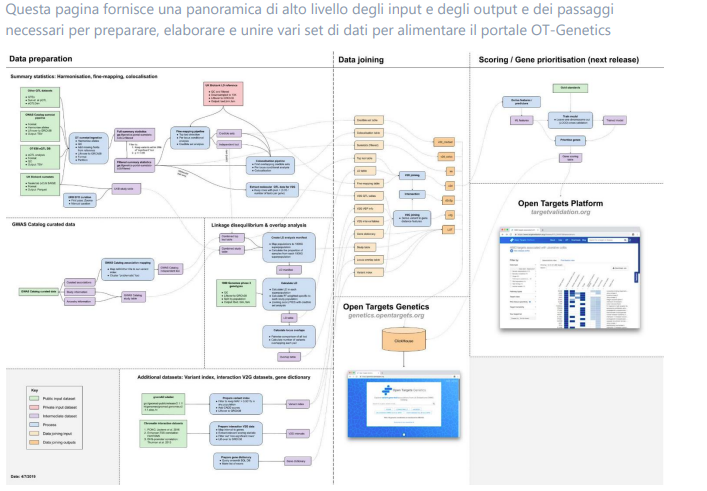
\includegraphics[width=0.85\textwidth]{figures/pipelines.png}
\end{center}


\subsection{Assigning Variants to Disease (V2D)}
Le associazioni variante-fenotipo che troviamo in letteratura sono state identificate tramite il catalogo NHGRI-EBI GWAS: data base curato manualmente di varianti pubblicate che soddisfano determinati criteri di inclusione dettati dal catalogo stesso.
In particolare, il catalogo GWAS estrae i dettagli sulle associazioni variante-fenotipo a un livello di significatività di $p \leq 1e{-5} (0.00001)$, tenendo presente che il valore p aiuta a capire se la differenza tra il risultato osservato e quello ipotizzato è dovuta alla casualità introdotta dal campionamento, oppure se tale differenza è statisticamente significativa, cioè difficilmente spiegabile mediante la casualità dovuta al campionamento.\\
\textit{\textbf{Nelle analisi di associazione genetica di tratti complessi, determinare la corretta soglia del valore di
 P per la significatività statistica è fondamentale per controllare il numero di associazioni di falsi positivi.}}\\
Il termine p-value sta ad indicare la probabilità che quanto stiamo sostenendo sia corretto con un piccolo margine di errore, oppure esso spiega che la probabilità di sbagliarsi è troppo alta per sostenere la veridicità di quello che ipotizziamo.
In OTG si includono le associazioni curate dal Catalogo GWAS con $p \leq 5e^{-8} (0.00000005)$.
I dati del repository delle statistiche di riepilogo del catalogo GWAS sono pertanto stati inclusi nel portale.\\
Oltre ai dati di derivazione del catalogo GWAS, si hanno a disposizione anche ampi archivi di statistiche riassuntive dai dati disponibili nella biobanca britannica.
\textbf{Questi dati sono sfruttati per scoprire i locus della malattia.}\\
Vengono usati due metodi per espandere le varianti associate alla malattia in un insieme più completo di varianti possibilmente causali:
[ricordando la differenza tra variant lead e variant tag: la VL è la variante].
\begin{enumerate}
    \item Espansione del LD utilizzando una popolazione di riferimento: questa viene applicata a tutti gli studi in OTG
        \subitem Le informazioni sul LD vengono calcolate utilizzando il pannello dell'aplotipo 1000 Genomes Phase 3 come riferimento
    \item Espansione mediante mappatura fine (analisi del set credibile), utilizzata dove sono disponibili statistiche riassuntive complete (attualmente i tratti della biobanca britannica e quelli inclusi nel riepilogo del catalogo GWAS archivio di statistiche).
\end{enumerate}


\subsection{Assigning Variants to Genes (V2G)}
Tutte le varianti nell'indice delle varianti vengono annotate utilizzando la pipeline di OTG V2G. la pipeline integra le prove V2G che rientrano in diversi tipi di dati principali:
\begin{itemize}
    \item Esperimenti sui loci dei tratti quantitativi del fenotipo molecolare (eQTL pQTL)
    \item Esperimenti di interazioni con cromatina
    \item In silico predizioni funzionali
    \item Distanza dal sito di inizio della trascrizione canonica
\end{itemize} 
All'interno di ogni tipo di dato ci sono molteplici fonti di informazioni prodotte da diversi metodi sperimentali.
Alcune di questi fonti possono essere ulteriormente suddivise tenendo conto di tessuti/cellule.\\
STEP DA SEGUIRE:
\begin{enumerate}
    \item \underline{\textbf{Pre-elaborazione}}
        \subitem{a.} \textbf{Filtraggio}: i set di dati grezzi vengono elaborati per conformarsi a un formato standard: si produce un file V2G.
        \subitem{b.} \textbf{Trasformazione del punteggio}: diverse fonti utilizzano metriche diverse per misurare l'associazione V2G: viene estratta quindi una metrica specifica dello studio pertinente seguita dalla trasformazione dei quantili utilizzando una distribuzione uniforme. I punteggi trasformati vengono arrotondati al decile più vicino.
    \item \underline{\textbf{Annotazione variante-gene}}: ogni coppia (V, G) è annotata con tutte le prove funzionali disponibili.
    \item \underline{\textbf{Punteggio}}: è stato sviluppato un sistema di punteggio in modo tale che per una data variante V possiamo ottenere un elenco di geni (G1, G2..) classificato in base a:
            \subsubitem{i.} Il punteggio V2G complessivo
            \subsubitem{ii.} Un punteggio V2G per sorgente
        \subitem{a.} \underline{AGGREGARE TRA LE CARATTERISTICHE}: Siccome alcune fonti di dati forniscono associazioni misurate in pi tessuti o linee cellulari, laddove esistono più funzionalità, le aggreghiamo prendendo il punteggio massimo su tutte le funzionalità per ciascun (V, G) coppia. Questa aggregazione fornisce un punteggio V2G per sorgente per ciascuno (V, G) coppia.
        \subitem{b.} \underline{AGGREGARE TRA LE ORIGINI}: La fase dopo combina le informazioni per produrre un punteggio complessivo V2G. attenzione: poiché alcune fonti possono essere più attendibili di altre, prima dell'aggregazione (con una conoscenza precedente) si ordinano le fonti in base all'attendibilità.
\end{enumerate}
\subsection{Prioritising causal genes at GWAS loci (L2G)}
\paragraph{Caratteristiche predittive} \textbf{L2G è un modello che da la priorità a probabili geni causali in ciascun locus GWAS in base alle caratteristiche genomiche genetiche e funzionali.} Le principali categorie di caratteristiche predittive sono (tenendo presente che abbiamo 51 caratteristiche predittive dalle 4 categorie qui sotto elencate):
\begin{itemize}
    \item Distanza (dalle varianti del set credibile al gene)
    \item Colocalizzazione molecolare dei QTL
    \item Interazione della cromatina
    \item Patogenicità varianti.\\
    Ogni set di dati di genomica funzionale fornisce punteggi da variante a gene $\rightarrow$ viene convertito il punteggio V-G in punteggi locus to gene, aggregando su varianti credibili identificate attraverso una mappatura fine.
\end{itemize}
\textbf{Per gli studi GWAS con statistiche riassuntive disponibili sono utilizzati insiemi credibili dalla mappatura fine approssimata dal fattore di Bayes, altrimenti sono utilizzati insiemi credibili basati su LD.}\\
Il modello L2G è distinto dalla pipeline V2G in quanto:
\begin{itemize}
    \item Utilizza un modello di apprendimento automatico per apprendere il peso di ciascuna fonte di prove basato su un gold standard di geni causali precedentemente identificati.
    Per consentire l'apprendimento automatico sono stati curati manualmente una serie di geni.
    \item Si basa su dati di mappatura fine e colocalizzazione.
\end{itemize}
Tener presente che alcune caratteristiche sono migliore nel predire il gene: vi è disponibile anche un grafico che indica l'importanza delle caratteristiche.
\paragraph{Interpretare il punteggio L2G}
Il modello produce un punteggio tra 0 e 1: questo può essere interpretato per dire che i geni con un punteggio L2G di 0.5 hanno una probabilità del 50\% di essere il gene causale nel locus.\\
\textbf{Attenzione:} è probabile che l'insieme di geni attualmente identificati come “causali” sia sbilanciato verso quelli che sono più vicini al picco GWAS $\rightarrow$ utile considerare non solo il punteggio, ma anche gli altri parametri disponibili.\\
Sono disponibili anche dei punteggi parziali: in particolari questi si trovano nella pagina GENE PRIORISATION per un locus. Qui oltre al punteggio complessivo troviamo anche quello parziale: si
tratta di una sottoanalisi in cui si prende in considerazione solo un insieme parziale di caratteristiche. Anche in questo caso il punteggio è compreso tra 0 e 1.\\
I punteggi L2G parziali sono utili per capire quanto sia forte l'evidenza per un dato gene basato su un singolo tipo di perditore, tenendo presente che questi modelli utilizzano meno info rispetto al modello completo.

\subsection{Colocalysasion Analysis}
Utilizzata per verificare se due segnali di associazione indipendenti in un locus sono coerenti con l'avere una variante causale condivisa. Se due tratti condividono una variante causale (= sono colocalizzati) ciò aumenta anche l'evidenza che condividano anche un meccanismo causale.\\
Si una analisi di colocalizzazione che per due tratti, integra l'evidenza su tutte le varianti al locus per valutare le seguenti ipotesi:
\begin{itemize}
    \item H0: Nessuna associazione con nessuno dei due tratti
    \item H1: Associazione con il tratto 1, non con il tratto 2
    \item H2: Associazione con il tratto 2, non con il tratto 1
    \item H3: Associazione con il tratto 1 e il tratto 2, due SNP indipendenti
    \item H4: Associazione con il tratto 1 e il tratto 2, un SNP condiviso
\end{itemize}
In questo quadro, l'evidenza per H4 è considerata evidenza per la colocalizzazione tra due tratti.




\section{Un esempio di utilizzo}
\subsection{Study}
\begin{box4}
    [title={\textbf{Ricerca per Studio}}]
    {Iniziamo la ricerca a partire dallo studio per:
    \begin{itemize}
        \item Visualizzare i loci associati a un tratto nello studio selezionato
        \item Identificare i geni prioritari implicati funzionalmente da ciascun locus
        \item Visualizzare il 95\% di set credibili (se disponibili) e proxy in ogni locus
    \end{itemize}}
\end{box4}
La prima cosa che visualizziamo sono le informazioni generali relative allo studio (il \textit{\textbf{summary}}), come l'ID di PUBMED, il numero di casi studiati, la grandezza dello studio ecc.
\begin{center}
    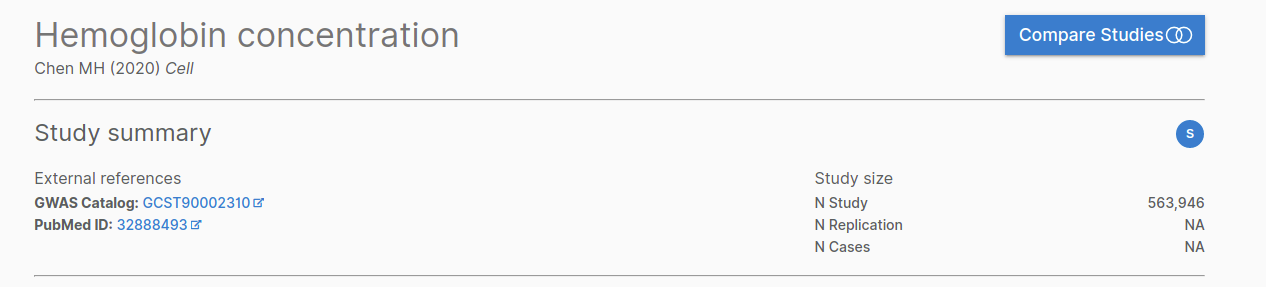
\includegraphics[width=0.85\textwidth]{figures/4-Study.png}
\end{center}
Subito dopo troviamo il primo plot: i loci associati indipendentemente sono riportati in un Manhattan plot semplificato. Sull'asse delle x vengono riportati i cromosomi, sull'asse delle y invece il p-value (in logaritmo).
\begin{center}
    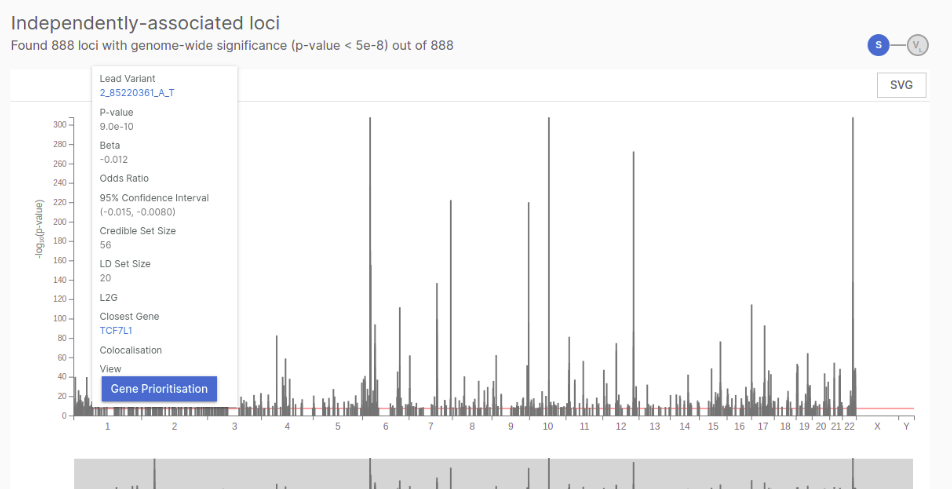
\includegraphics[width=0.85\textwidth]{figures/5-Study.png}
\end{center}
I dettagli completi di ogni locus sono riassunti nella tabella sotto il Manhattan plot. Il gene con il punteggio più alto è definito come il gene con il maggior peso di prove funzionali tra tutte le fonti e i tipi di cellule che lo collegano al locus specificato direttamente o tramite una Variant Tag. 
\begin{center}
    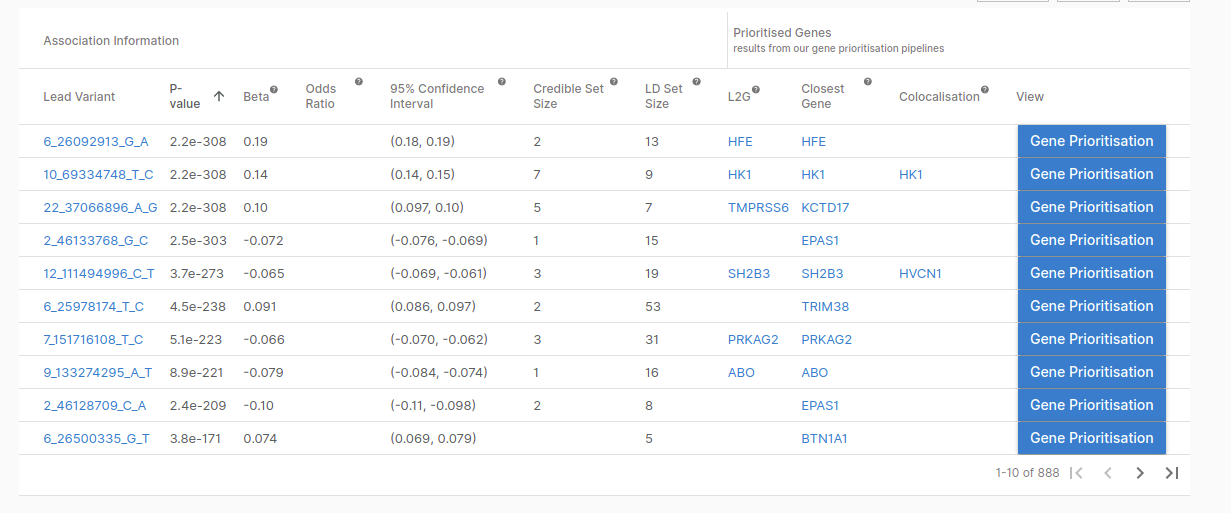
\includegraphics[width=0.85\textwidth]{figures/6-Study.png}
\end{center}
\subsubsection{Compare Studies}
Dalla pagina Studio, è possibile confrontare rapidamente più studi per identificare segnali sovrapposti: \textbf{Compare Overlapping Studies}.\\
Il primo studio verrà caricato nella vista di confronto come root, con i loci riportati a significatività dell'intero genoma, plottati in base alla posizione. Solo gli studi con almeno un locus sovrapposto verranno visualizzati come opzione di confronto. Gli studi nel menù a tendina sono ordinati in maniera decrescente in base al numero di sovrapposizioni con la radice caricata.
\begin{center}
    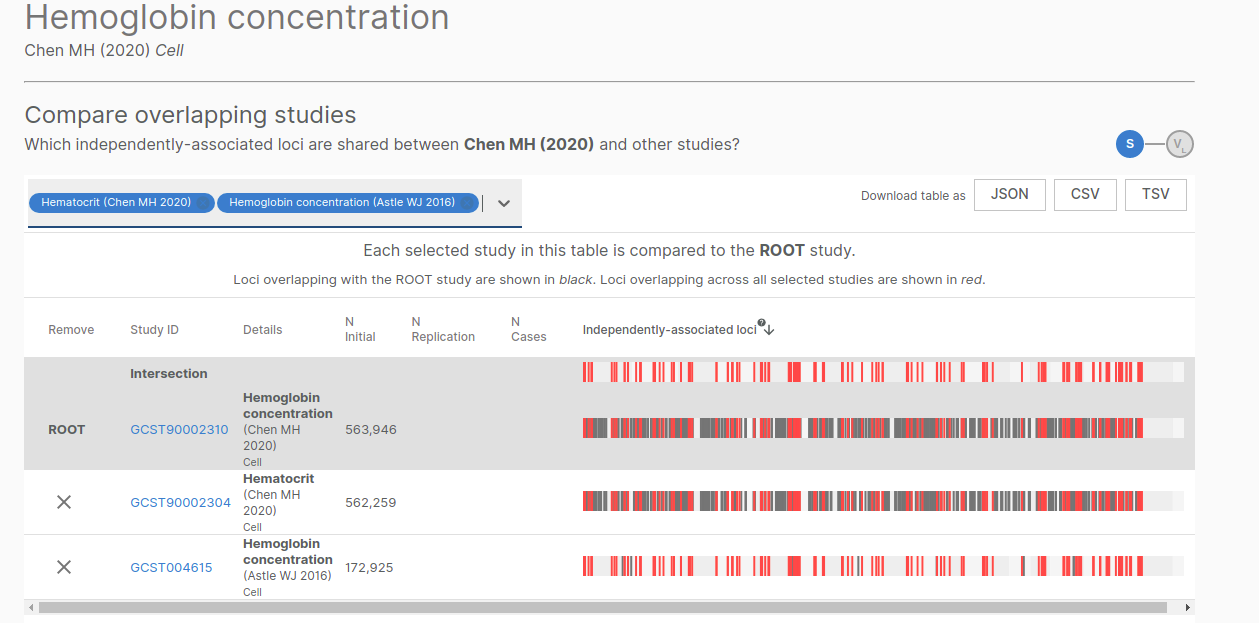
\includegraphics[width=0.85\textwidth]{figures/7-Compare Studies.png}
\end{center}
Quando viene caricato più di uno studio (come in questo caso), loci intersecanti di tutti gli studi caricati vengono visualizzati in rosso sia sulla barra di intersezione nella parte superiore della vista, sia all'interno di ogni studio. I loci all'interno di ogni studio che si sovrappongono allo studio radice vengono visualizzati in nero. I loci non sovrapposti sono tracciati in grigio.\\
Sotto la visualizzazione del grafico, ogni locus sovrapposto in tutti gli studi caricati è riassunto in una tabella.
\begin{center}
    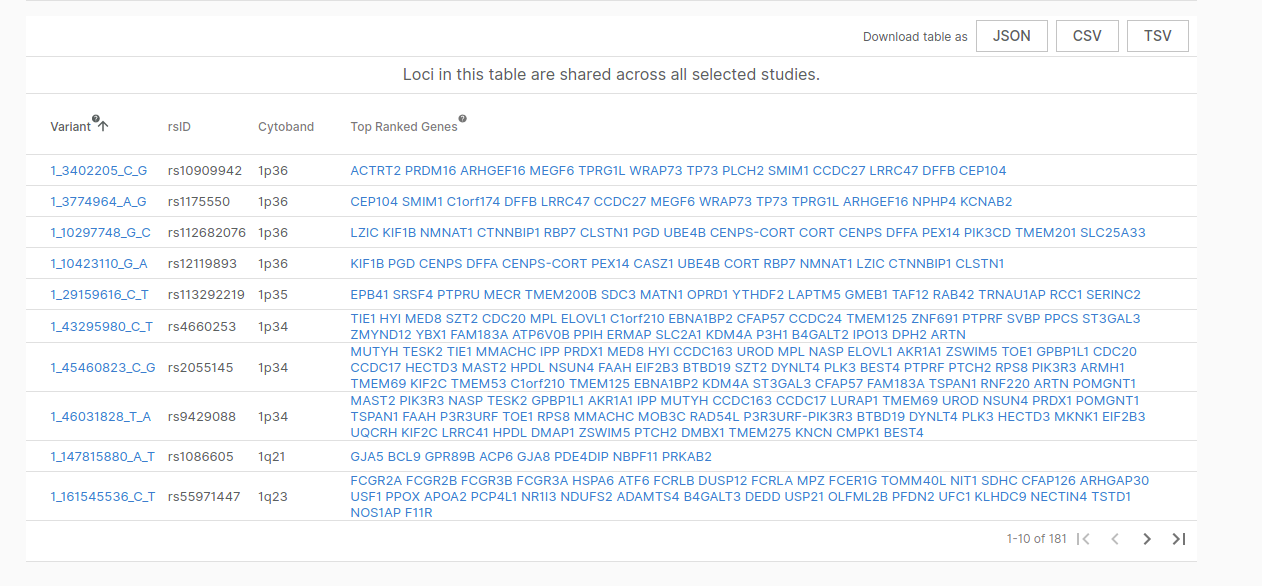
\includegraphics[width=0.85\textwidth]{figures/8-Compare Studies.png}
\end{center}
I geni con il punteggio più alto visualizzati sono i geni principali implicati direttamente dalla Lead Variant mostrata e non tengono conto dei geni assegnati a nessuna Tag Variant della Lead. Potrebbe quindi esserci un elemento di mancata corrispondenza tra il gene mostrato qui e il gene funzionale previsto nel locus.
\subsection{Variant}
\begin{box4}
    [title={\textbf{Ricerca per Variante}}]
    {Iniziamo la ricerca a partire dalla variante per:
    \begin{itemize}
        \item Identificare un elenco classificato di geni funzionalmente implicati dalla variante
        \item Visualizzare e analizzare i dati funzionali mediante i quali i geni sono assegnati a questa variante
        \item Visualizzare i risultati PheWAS per la variante nella biobanca britannica
        \item Visualizzare la struttura del collegamento intorno alla variante
    \end{itemize}}
\end{box4}
Anche in questo caso per prima cosa vedremo le informazioni generali riguardo alla variante, che essa sia Lead o Tag le informazioni variano molto poco.
\begin{center}
    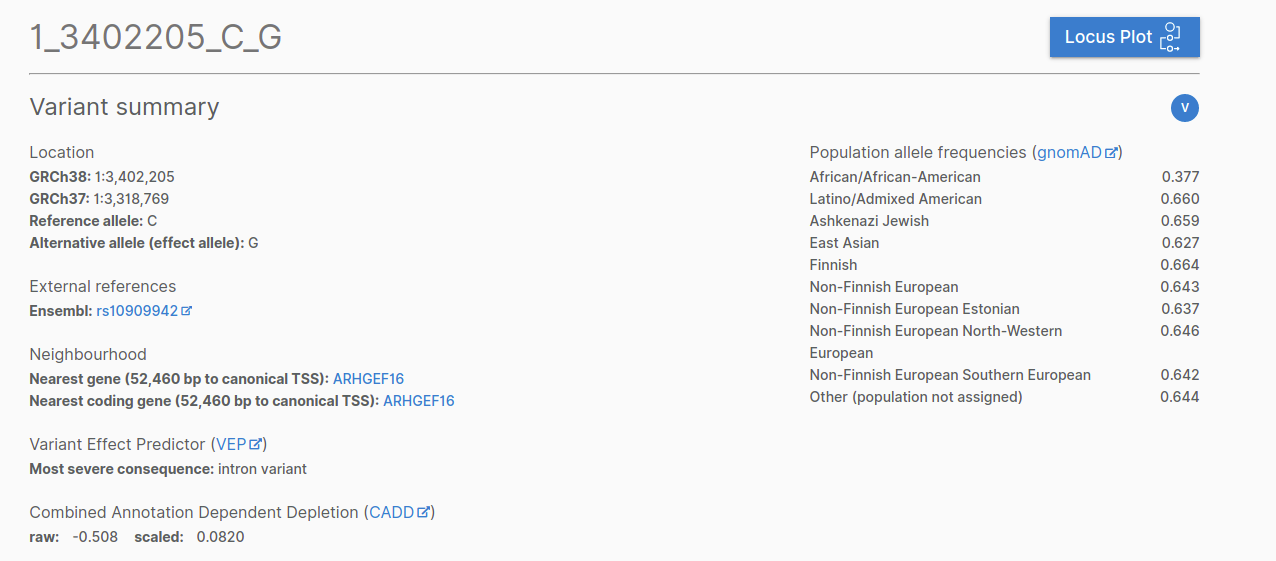
\includegraphics[width=0.85\textwidth]{figures/9-Variante.png}
\end{center}
Subito sotto troviamo la tabella \textbf{Assigned Genes}, che riassume l'entità delle prove con cui la variante interrogata implica vari geni. 
\begin{center}
    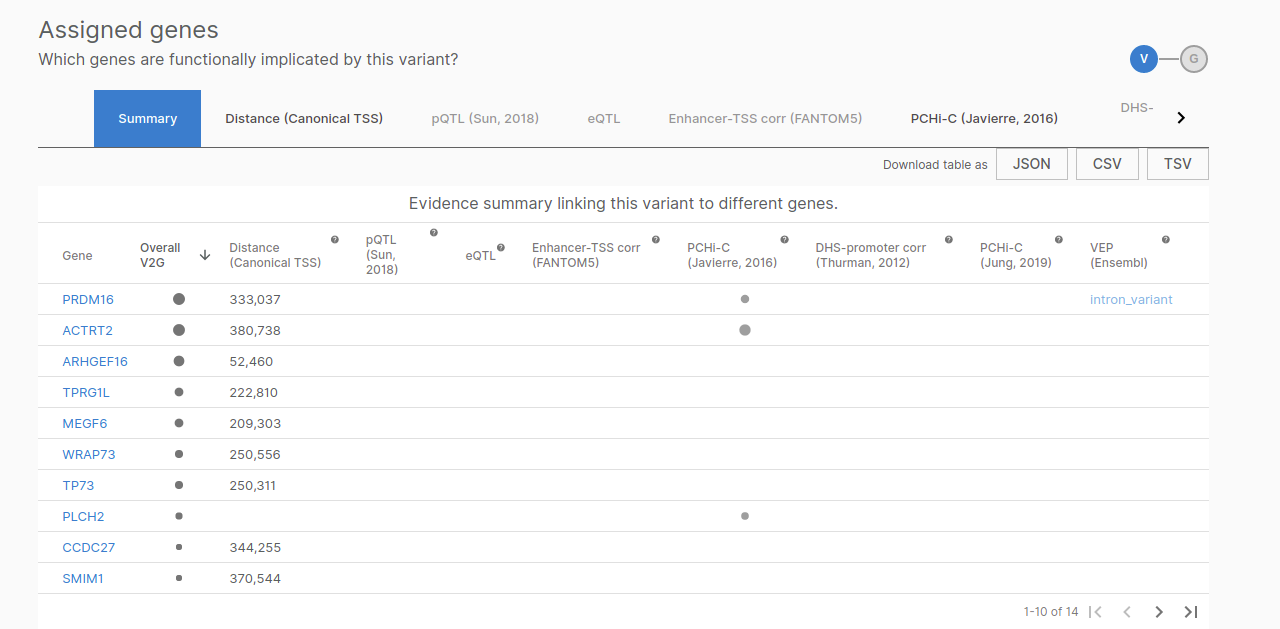
\includegraphics[width=0.85\textwidth]{figures/10-Variante.png}
\end{center}
La visualizzazione predefinita riepiloga le prove combinate per ciascun gene per ciascuna origine dati funzionale, compresse tra i tipi di cellule all'interno dell'origine dati. Il G2V complessivo è una rappresentazione di questa ponderazione combinata delle prove per ciascun gene. 
La presenza di un \textbf{pallino} nella tabella indica che vi sono prove dalla data fonte di dati che collegano il gene alla variante interrogata, in almeno un tipo di cellula.
Per visualizzare le prove specifiche del tessuto all'interno di un'origine dati, selezionare l'origine dati dalle schede visibili nella parte superiore del widget della tabella. Verrà aperta una vista equivalente segregata per tipo di cella anziché per origine dati, come sopra per le prove eQTL. Se l'evidenza dell'origine dati in esame può essere interpretata in modo direzionale, i proiettili verranno colorati in base alla direzione dell'effetto.\\
Subito sotto troviamo la sezione che presenta gli studi che collegano, con la variante in esame, determinati \textbf{PheWAS}. 
\begin{center}
    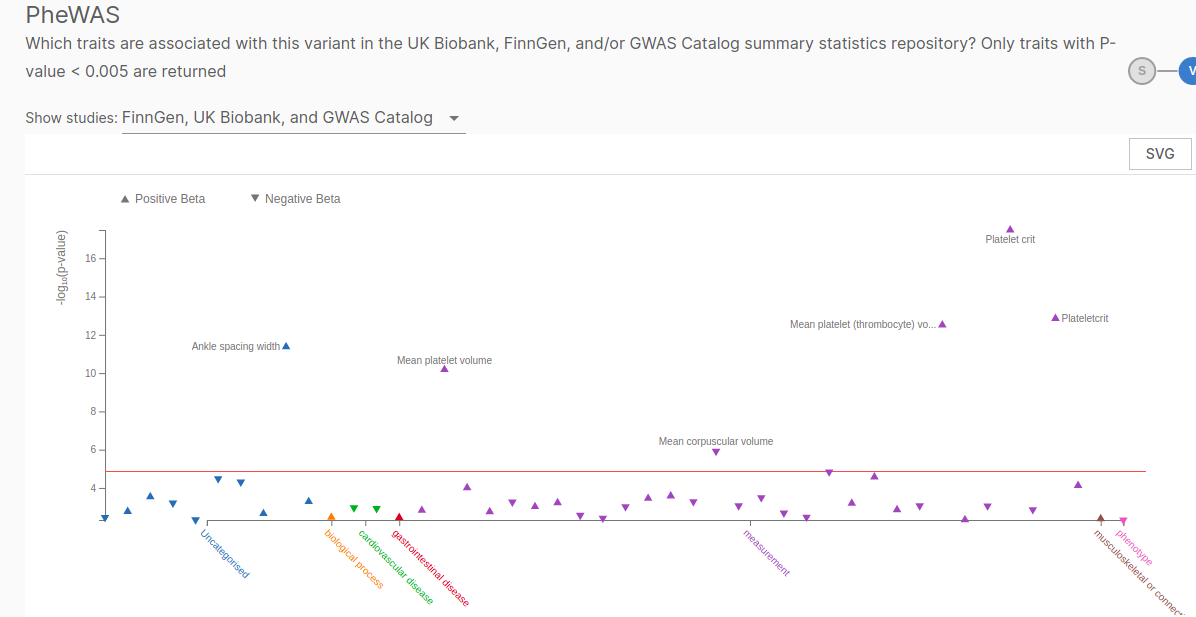
\includegraphics[width=0.85\textwidth]{figures/11-Variante.png}
\end{center}
I risultati di PheWAS per la variante selezionata in tutti i fenotipi della BioBank del Regno Unito, vengono visualizzati come un grafico PheWAS segregato per raggruppamento di fenotipi di alto livello e dettagliato in una tabella sottostante.\\
\begin{center}
    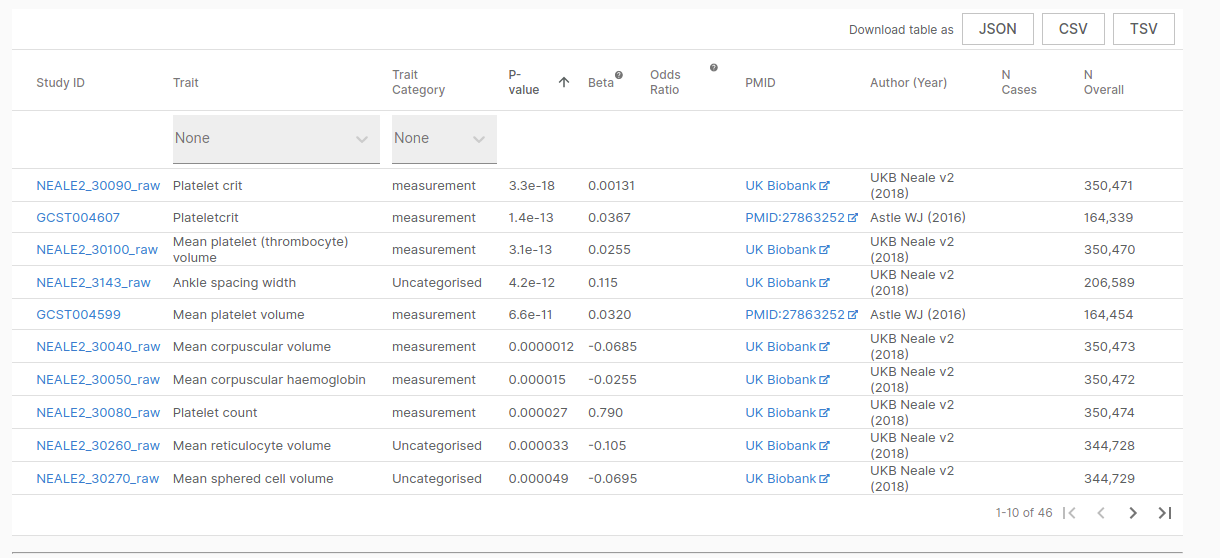
\includegraphics[width=0.85\textwidth]{figures/13-Variante.png}
\end{center}
La direzione della freccia corrisponde alla direzione dell'effetto beta e i punti sono colorati in base al loro fenotipo ampio.
Infine, vengono visualizzate due tabelle dedicate all'architettura genetica del locus a cui appartiene la variante di interesse - 'GWAS Lead Variants' e 'Tag Variants'. Il primo mostra tutte le varianti di lead GWAS (dal catalogo GWAS o dalla biobanca britannica) a cui la variante interrogata è stata assegnata come proxy (tag) in base a LD o fine-mapping. Se la variante interrogata è essa stessa una variante lead GWAS, la seconda tabella mostra tutte le varianti che le sono state assegnate come proxy. Questa tabella non verrà visualizzata se la variante interrogata non è una variante lead.
\subsection{Gene}
\begin{box4}
    [title={\textbf{Ricerca per Gene}}]
    {Iniziamo la ricerca a partire dal gene per:
    \begin{itemize}
        \item Identificare i loci che implicano funzionalmente un gene
        \item Collegarti a informazioni dettagliate sul gene e sui farmaci che lo prendono di mira
        \item Identificare in quali tratti questo gene può svolgere un ruolo, in base alle varianti a cui è assegnato
    \end{itemize}}
\end{box4}
La ricerca porta alle principali informazioni sul gene e collega a vari link sulla piattaforma Open Targets Platform:
\begin{center}
    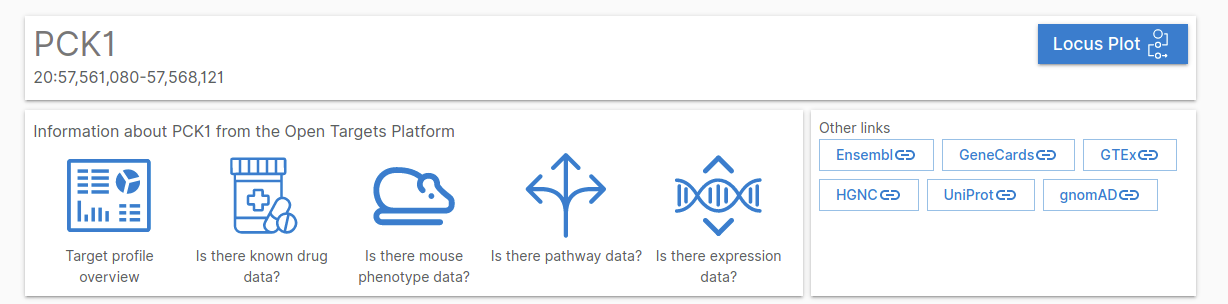
\includegraphics[width=0.85\textwidth]{figures/1-Gene.png}
\end{center}
accanto ci sono altri link. E sopra il link per collegarsi al Locus Plot, che vedremo in seguito.
Subito sotto troviamo la sezione \textbf{Associated studies}, tratta dalla \textit{locus-to-gene pipeline}.
\begin{center}
    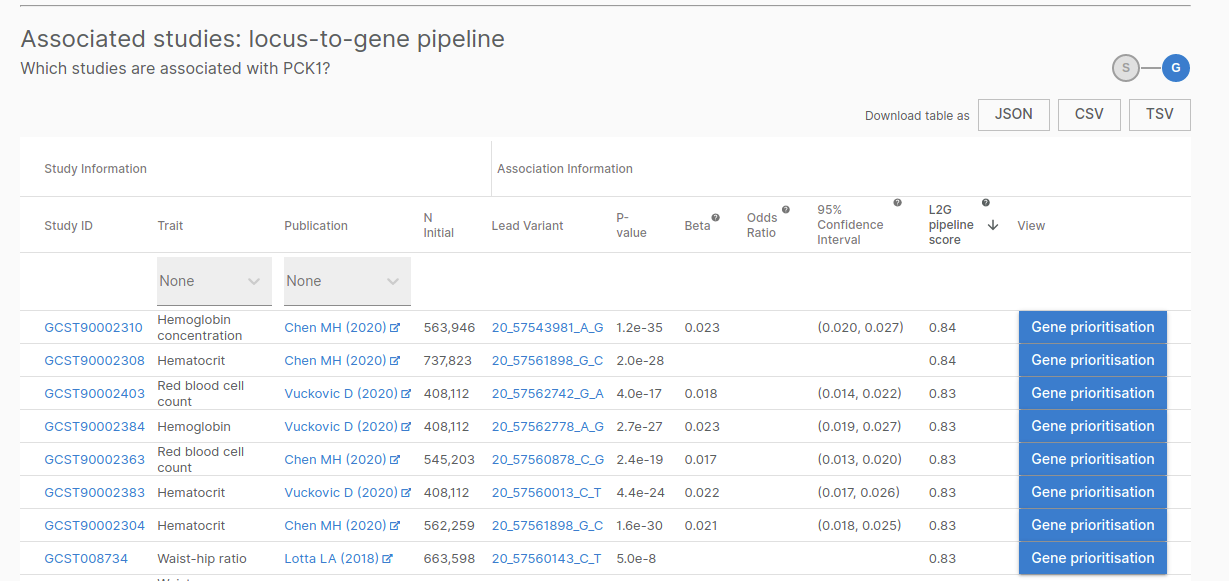
\includegraphics[width=0.85\textwidth]{figures/2-Gene.png}
\end{center}
La tabella associa gli studi e i fenotipi, da UKB, che sono associati con il gene di cui stiamo visualizzando la pagina. Un gene è connesso a un tratto nei casi in cui il gene è stato funzionalmente assegnato a un locus associato a questo tratto, tramite la Variant Lead o tramite una proxy Variant Tag assegnato. Accanto ci riporta al link \textbf{Gene Priorisation}, che vedremo in seguito.\\
Subito dopo abbiamo altri Studi associati, ma questa volta tramite la \textit{\textbf{colocalisation analysis}}, che risponde alla domanda: quali studi hanno evidenze di colocalizazione con qtl molecolari per il gene in questione?
\begin{center}
    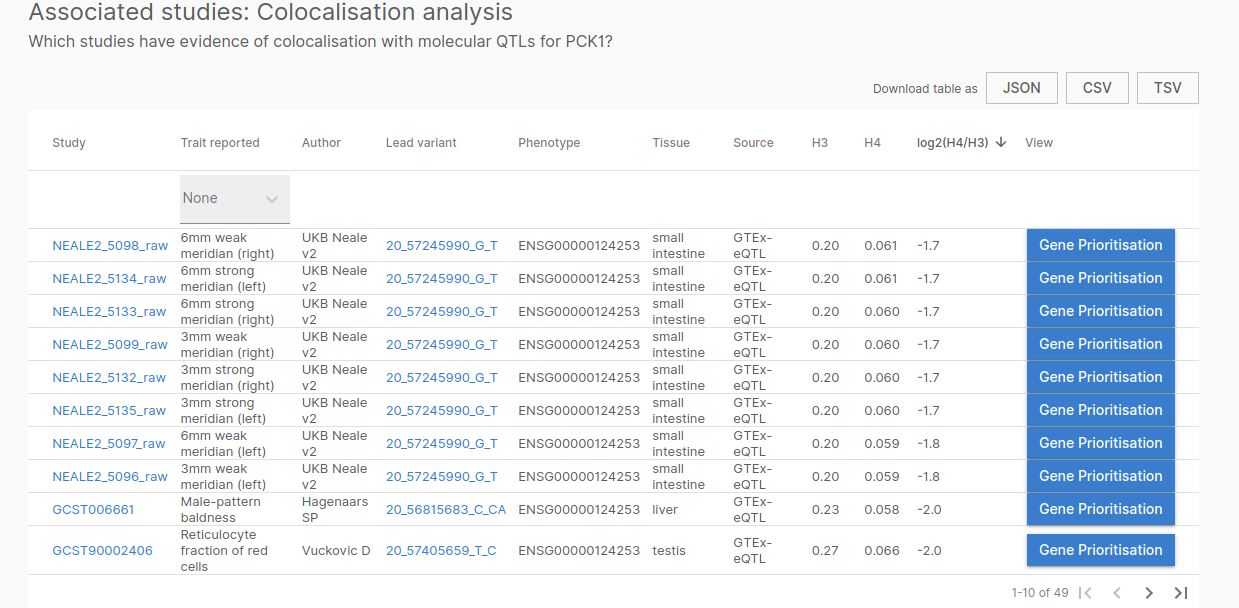
\includegraphics[width=0.85\textwidth]{figures/3-Gene.png}
\end{center}
\subsubsection{Gene Priorisation}
In questa pagina stiamo studiando la malattia selezionata, nel locus suscettibile, possiamo ad esempio capire se l'allele alternativo è protettivo oppure no.
Questa pagina è chiamata "Study-Locus" e vi si può accedere da Gene e da Studio. Qui si investiga una specifica Lead Variant e un GWAS study.\\
Dapprima abbiamo la informazioni di base: ad esempio tramite l'odds ratio capiamo se l'allele alternativo è associato ad un alto o basso rischio della malattia su cui si concentra lo studio.Tutte le dimensioni degli effetti sono in relazione all'allele alternativo, che è l'allele riportato ultimo nell'ID della variante.
\begin{center}
    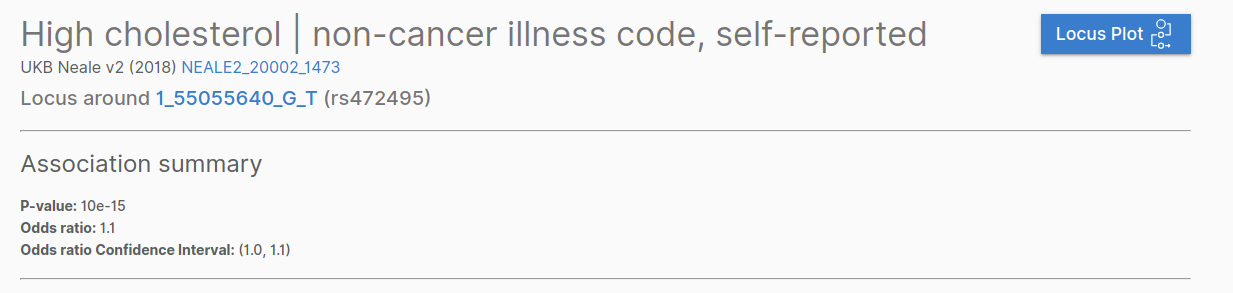
\includegraphics[width=0.85\textwidth]{figures/StudyLocus.png}
\end{center}
Subito sotto una tabella riporta i geni prioritizzati tramite la \textbf{Locus To Gene Pipeline}.
\begin{center}
    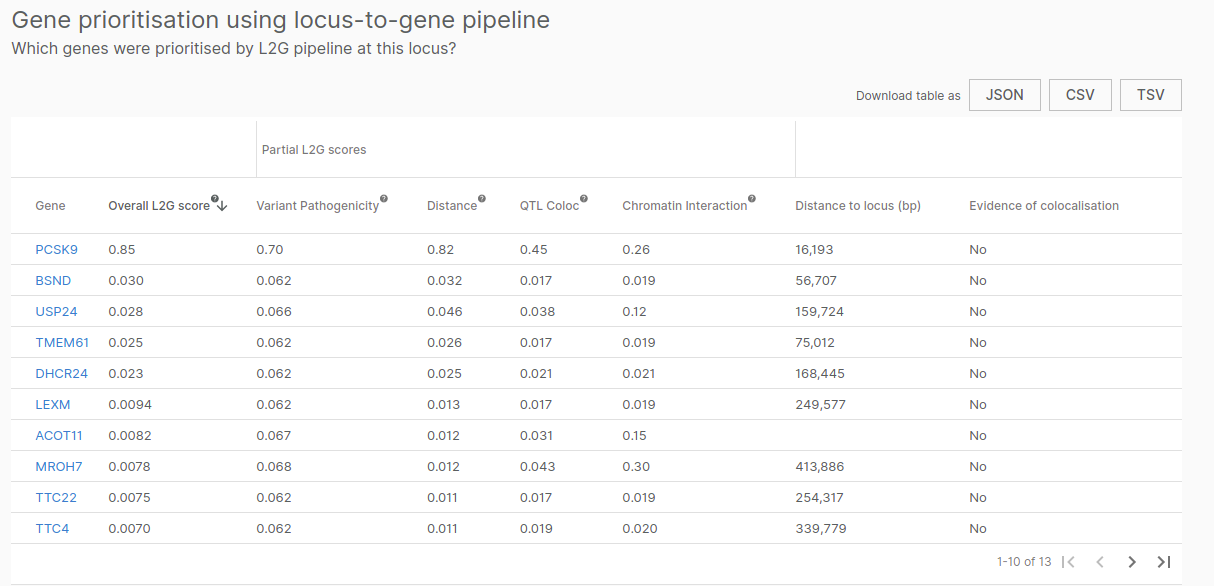
\includegraphics[width=0.85\textwidth]{figures/StudyLocus2.png}
\end{center}
Questi sono ordinati tramite lo score assegnato appunto dalla pipeline, riportando anche tutte le features usate per fare il training del modello che ha effettuato la prioritizzazione (quindi distanza, colocalizzazione dei QTL, ecc.). Alla luce dei dati troviamo anche la risposta alla domanda: \textbf{“L'assegnamento del gene è supportato da evidenze di colocalizzazione?”}
Subito dopo visualizziamo sempre informazioni riguardanti la prioritizzazione dei geni, ma ottenute tramite la colocalisation Analysis Pipeline: la colocalizzazione dei geni principali, ottenuti mediante la L2G pipeline, in diversi tessuti è mostrata in una heatmap e in una tabella.
\begin{center}
    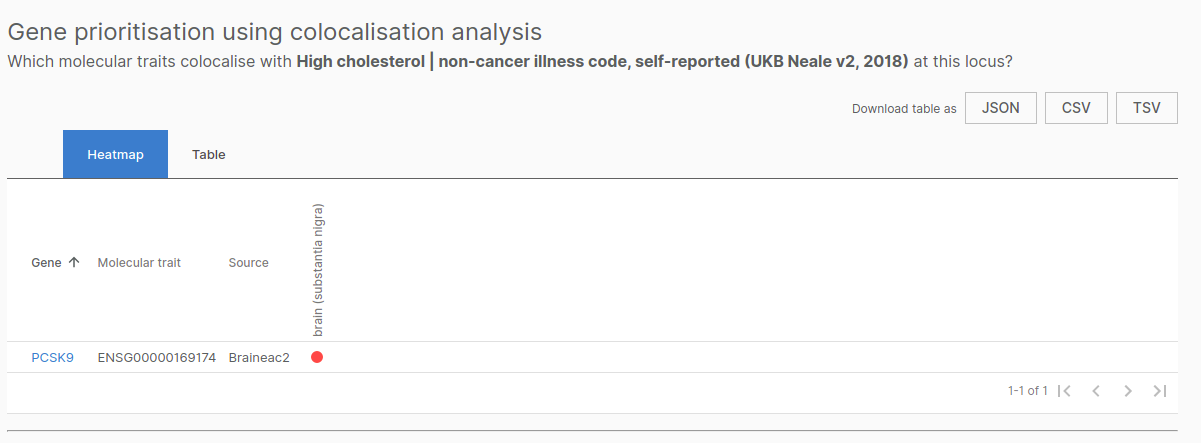
\includegraphics[width=0.85\textwidth]{figures/StudyLocus3.png}
\end{center}
Nella tabella la QTL beta è per la variante che stiamo visualizzando, più che per tutte quelle riportate. Questo permette di comparare la direzione degli effetti nei diversi tessuti o geni nei tessuti, così da poter rimanere consistenti attraverso tutti gli studi.\\
Sotto, la tabella \textbf{GWAS Study Colocalisation}, mostra la colocalizzazione tratto-incrociata. Lo "Study beta" è sempre per la variante all'inizio della pagina. 
\begin{center}
    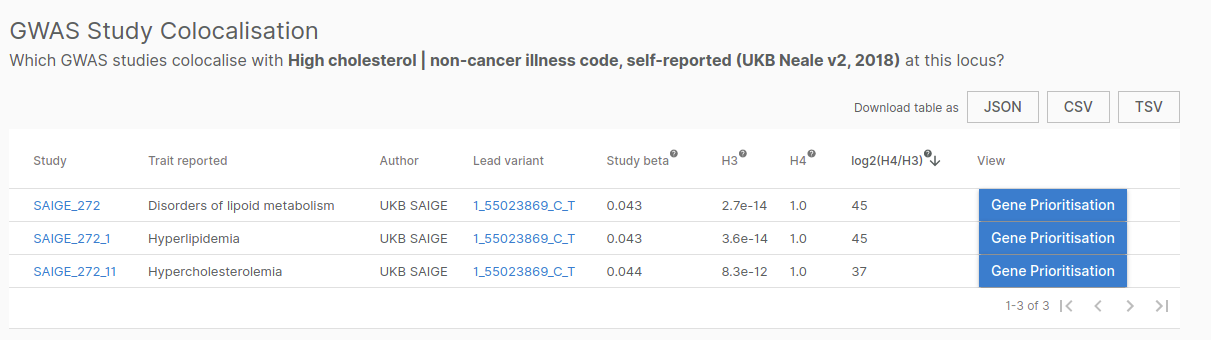
\includegraphics[width=0.85\textwidth]{figures/StudyLocus4.png}
\end{center}
La sezione finale fornisce l'insieme delle probabili varianti causali (set credibili) a questo
locus: \textbf{Credible Set Overlap} mostra il fine mapping dei set credibili attraverso più studi. Il primo è lo studio analizzato nella pagina:
\begin{center}
    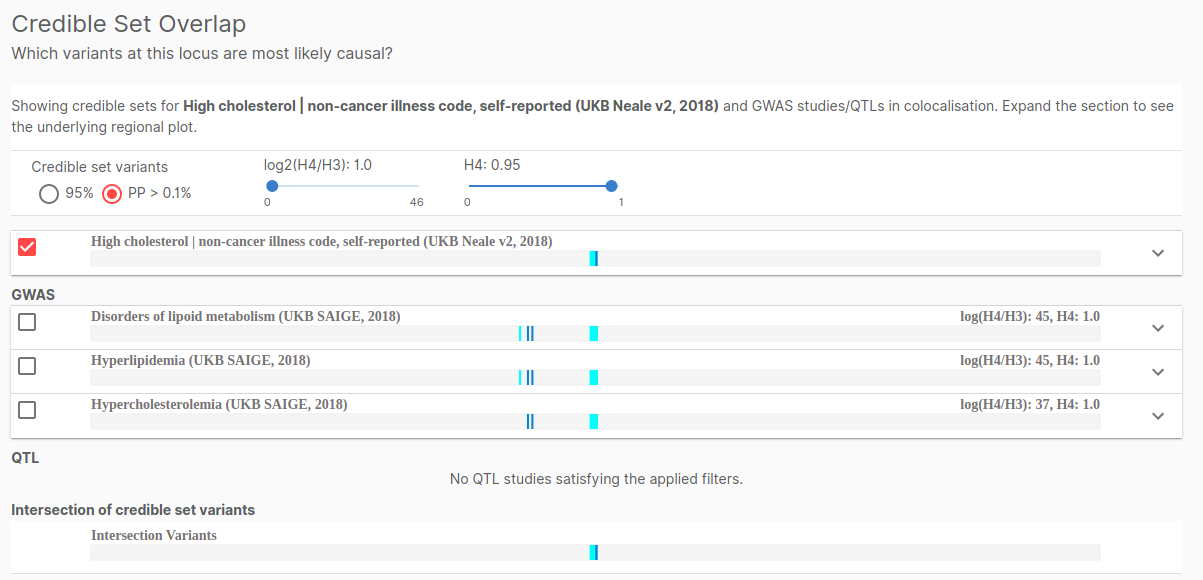
\includegraphics[width=0.85\textwidth]{figures/StudyLocus5.png}
\end{center}
Sono evidenziati le varianti che rientrano nel set credibile al 95\% o con una probabilità a posteriori maggiore dello 0.1\%. \\
Le freccette in basso accanto agli studi consentono agli utenti di visualizzare un grafico regionale di base per le consultare le statistiche di riepilogo. Vengono visualizzate anche le tracce per gli studi che colocalizzano: se due o più studi colocalizzano, è più probabile che condividano una variante causale, quindi confrontando i set credibili per gli studi di colocalizzazione, potremmo essere in grado di perfezionarli.
Selezionando più tracce, nella tabella sotto l'elenco degli studi, si possono visualizzare le intersezioni di varianti nei set credibili.
\begin{center}
    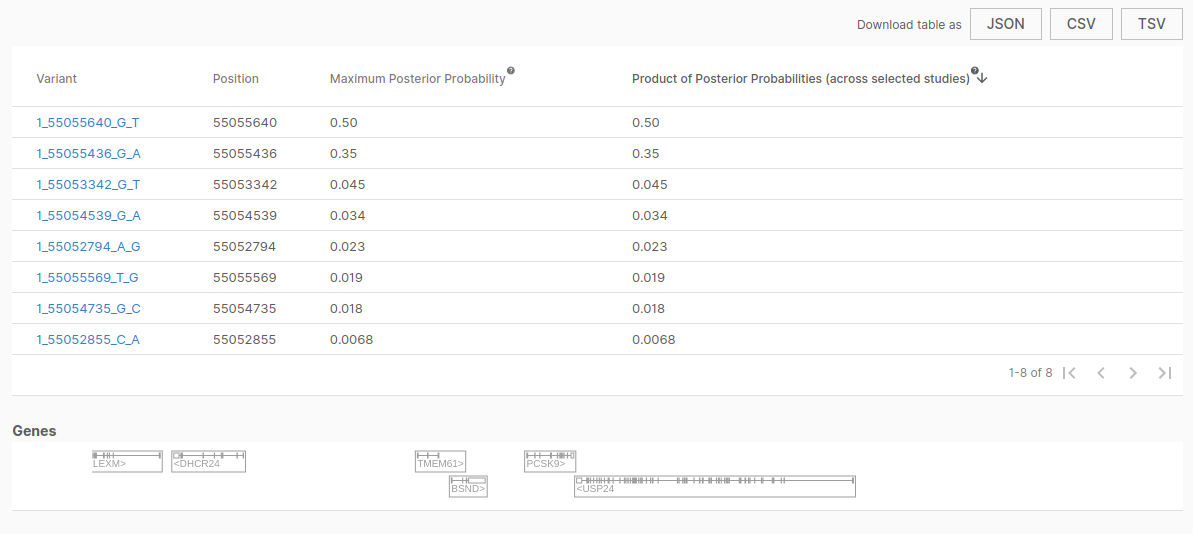
\includegraphics[width=0.85\textwidth]{figures/StudyLocus6.png}
\end{center}
\subsection{Locus Plot}
L'ultima sezione è una delle più interessanti, si tratta del Locus Plot:  accessibile da tutte e 4 le query (Study, Variant Lead, Variant Tag e Gene) e riporta, se si accede da una variante, se è in visualizzazione Lead o Tag.
\begin{center}
    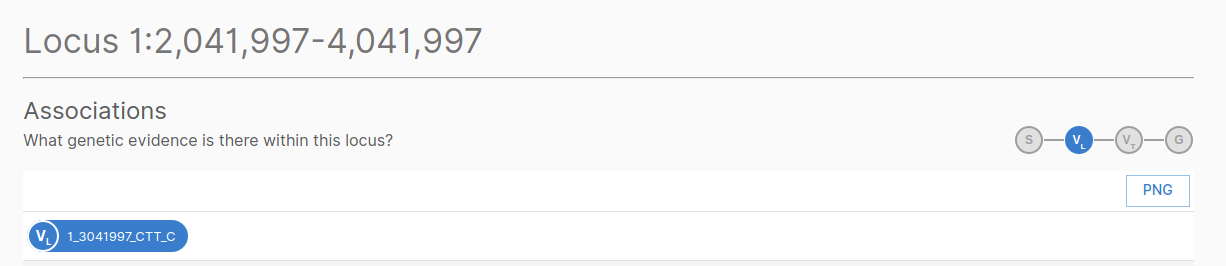
\includegraphics[width=0.85\textwidth]{figures/16-LocusPlot.png}
\end{center}
È progettato per riassumere efficacemente la complessità dei collegamenti tra numerosi geni (bersagli), tratti e lead variants. Il Locus Plot utilizza un browser track-style per visualizzare un locus che può essere centrato su un gene, una variante o un tratto di interesse (ognuno noto come entità). Tratti di collegamento, varianti e geni sono stringhe di prova che indicano un'associazione o un collegamento funzionale tra le entità.
\begin{center}
    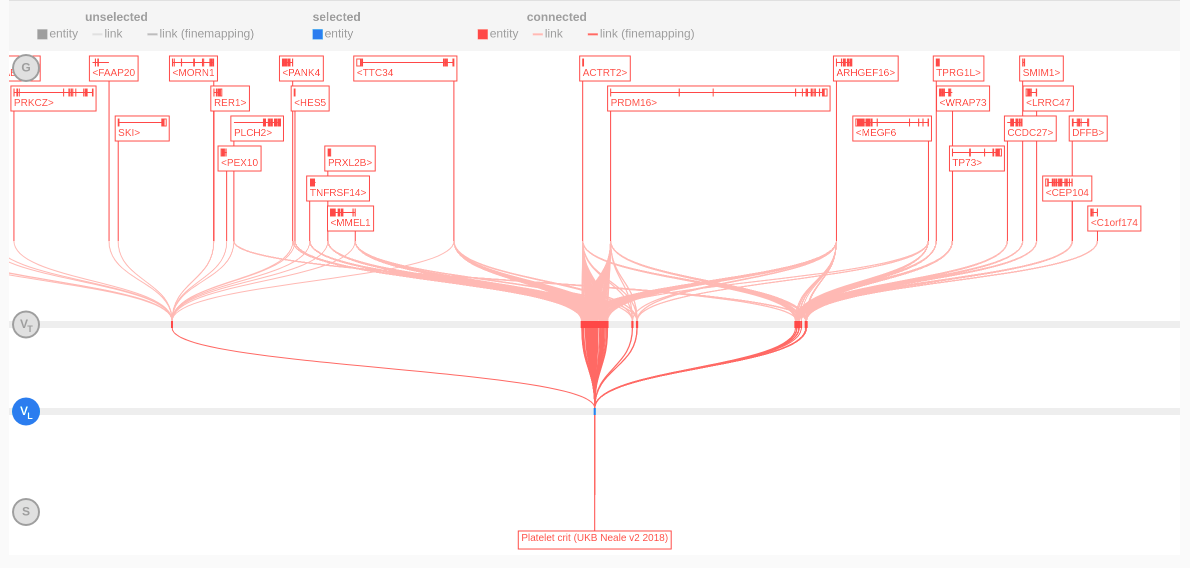
\includegraphics[width=0.85\textwidth]{figures/17-LocusPlot.png}
\end{center}

\section{Possibili domande}
\paragraph{Che differenza c'è tra Varianti Lead e Tag?}
Inanzitutto Open Targets è un portale di genetica concentrato sulle varianti. Le varianti lead si trovano dall'annotazione basata su dati curati manualmente del catalogo GWAS e dati provenienti dalla BioBanca britannica. 
La variant lead è la variante leader che guida nella ricerca, ma non si può dare per scontato che questa sia la variante causale, ovvero quella responsabile di un effetto biologico sul fenotipo. Per questo motivo si cerca di prendere in considerazione un più ampio set di variabili potenzialmente causali, che chiamiamo tag variants e che otteniamo da due tipologie di espansione: 
\begin{itemize}
    \item LD expansion (se la VL è presente nel pannello di riferimento) : sappiamo che il genoma viene ereditato a blocchi e ogni blocco è definito da un aplotipo, che a sua volta è definito da un insieme di SNPs. OTG prende in considerazione il LD perchè pazienti che hanno ereditato lo stesso segmento cromosomico, definito dal medesimo aplotipo, possono aver ereditato anche la stessa mutazione. Il LD ha persmesso nelle analisi di associazioni, si studiare soo gli SNPs necessari a identificare il blocco di DNS in disequilibrium. 
    \item  Espansione per fine-mapping : identifica quali varianti hanno maggiore probabilità di essere causali ( = responsabili dell’associazione)
\end{itemize}
\paragraph{Cos'è la Colocalizzazione?}
L'analisi di colocalizzazione viene utilizzata per verificare se due segnali di associazione indipendenti in un locus hanno una variante causale condivisa. Se due tratti condividono una variante causale (sono colocalizzati), ciò aumenta l'evidenza che condividono anche un meccanismo causale. 
 Esempio: se il segnale di una malattia e il livello proteico (pQTL) si colocalizzano, ciò può fornire la prova del ruolo della proteina nel causare la malattia.
\paragraph{Cos'è la Prioritizzazione?}
La Prioritizzazione di geni è il processo di assegnazione della probabilità del coinvolgimento del gene nella generazione di un fenotipo di malattia. Questo approccio restringe e organizza in ordine di probabilità nel coinvolgimento della malattia, l'insieme di geni da testare sperimentalmente. 
La prioritizzazione in OTG permette di dare supporto al portale OTP. 

\paragraph{Qual è la differenza tra GWAS e PheWAS?}
Sono due tipologie di studio differente:
\begin{itemize}
    \item Un PheWAS inizia con una variante genetica di interesse e analizza sistematicamente molti fenotipi (cioè, "a livello di fenotipo") per l'associazione al genotipo. È l'abbreviazione di \textit{studio di associazione sull'intero fenomeno}: uno studio in cui l'associazione tra polimorfismi a singolo nucleotide o altri tipi di varianti del DNA viene testata su un gran numero di fenotipi diversi.
    \item Come spiegato in precedenza invece uno \textit{studio di associazione sull'intero genoma} (GWAS) è un approccio utilizzato nella ricerca genetica per associare variazioni genetiche specifiche a particolari malattie. Il metodo prevede la scansione dei genomi di molte persone diverse e la ricerca di marcatori genetici che possono essere utilizzati per prevedere la presenza di una malattia.
\end{itemize}
\paragraph{Come sono definiti gli Overlap nella pagina del Compare Studies?}
Per definire la sovrapposizione per una data Lead Variant $x$, le Tag Variants, definite da LD-expansion di $x$ sono incrociate con le Tag Variants di tutte le Lead Variants entro 5 mB da $x$. In ogni caso, quando una Tag Variants di $x$ è condivisa con un'altra Lead Variants, tale Lead è considerata parte dello stesso segnale di $x$. Ogni locus condiviso, quindi, può essere considerato come un insieme di segnali che occupano un aplotipo comune.
\paragraph{Come si legge il Manhattan Plot?}
La linea rossa è la linea di significatività genome-wide.\\
Si può passare il mouse su un locus per visualizzarne i dettagli, incluso il gene più classificato per il locus secondo la pipeline di Open Targets Genetics. Selezionando un cromosoma, dal menù a discesa o facendo clic sul numero del cromosoma sull'asse x, la visualizzazione dei loci situati su quel cromosoma verrà ampliata e ingrandita e verranno limitati i dettagli dei loci visualizzati nella tabella allegata, di seguito. Vengono fornite le opzioni per scaricare il plot come vettore.
\paragraph{Come si legge il Plot dei PheWAS?}
La linea rossa denota il livello di significatività dopo la correzione di Bonferroni per il numero di fenotipi testati, considerandoli prudentemente indipendenti. Ogni fenotipo è rappresentato da un triangolo nel plot: la direzione del traingolo corrisponde alla direzione dell'effetto beta ed è colorato in base al suo "fenotipo ampio". I dettagli dell'associazione di ciascun fenotipo con il tratto di interesse sono visualizzati in una tabella sotto il grafico, che può essere ordinata, filtrata su colonna e scaricata. Per ciascun fenotipo viene fornito anche un collegamento alla vista locus diretta, che caricherà la vista locus con la variante e il tratto UK Biobank preselezionati.
\paragraph{Quali sono le "tecnologie recenti" menzionate nell'approccio innovativo di OTG?}
Partendo dai GWAS e dai più recenti dati di trascrittomica e proteomica, che appartengono alla BioBank, e quindi dai database più recenti e aggiornati (su cui si appoggia OTG rimanendo costantemente aggiornato), fino ad arrivare alle pipeline usate (di cui parleremo brevemente in seguito perché molto tecniche ed esulano dal portale in sé per sé su cui ci siamo concentrate)
\paragraph{Come viene creata l'informazione contenuta nel database?}
Tutte le pipeline sono interne ad OTG, non sono esterne, ma proprie del databse.
\paragraph{Di che tipo sono i campioni contenuti nel database?}
OTG si basa principalmente su campioni europei, basandosi sulla UK BioBank. Non è stata trovata al momento una fonte di campioni differenti, che mantenga la stessa qualità, ma la piattaforma sta lavorando per ampliare i campioni e cercarne una adeguata.
%Se più di un gene viene valutato allo stesso modo in questo locus, vengono visualizzati tutti i geni con il punteggio massimo. Se lo studio selezionato dispone di statistiche complete disponibili, la dimensione del set credibile per ciascun locus viene visualizzata accanto al numero di Variant Tag.
\paragraph{Cosa intendete quando parli di dati senza statistiche riassuntive dal catalogo GWAS, curati manualmente? Quali sono le statistiche riassuntive?}
Le statistiche riassuntive sono i valori di p aggregati e i dati di associazione per ogni variante analizzata in uno studio di associazione sull’intero genoma.\\
Non sempre i GWAS forniscono questi dati, è per questo che ottenendo dati senza statistiche aggiuntive è necessario integrarle alle Tag Variants.
\paragraph{Cosa intendi con Linkage Disequilibrium espansione?}
Sappiamo che il genoma viene ereditato a blocchi e ogni blocco è definito da un aplotipo, che a sua volta è definito da un insieme di SNPs. OTG prende in considerazione l'LD perchè pazienti che hanno ereditato lo stesso segmento cromosomico, definito dal medesimo aplotipo, possono aver ereditato anche la stessa mutazione. L'LD ha persmesso nelle analisi di associazioni, di studiare soo gli SNPs necessari a identificare il blocco di DNS in disequilibrium. 
\paragraph{Qual è la differenza tra 1$\_$55039974$\_$G$\_$T e rs11591147?}
Entrambe le nomenclature fanno riferimento a una variante, mentre la prima ha una forma cromosoma$\_$posizione$\_$riferimento$\_$alternativo, la seconda rappresenta il nome. 
\end{document}